\documentclass[]{article}

\usepackage[margin=1.0in]{geometry}
\usepackage{graphicx}
\usepackage{float}
\usepackage{amsmath}
\usepackage{amssymb}
\usepackage{hyperref}

\pagestyle{plain}

% scale:
% 0.161
% 0.126
% 0.126

% 0.161
% 0.126
% 0.126
\begin{document}
%\begin{minipage}{6in}
%\centering
%\raisebox{-0.5\height}{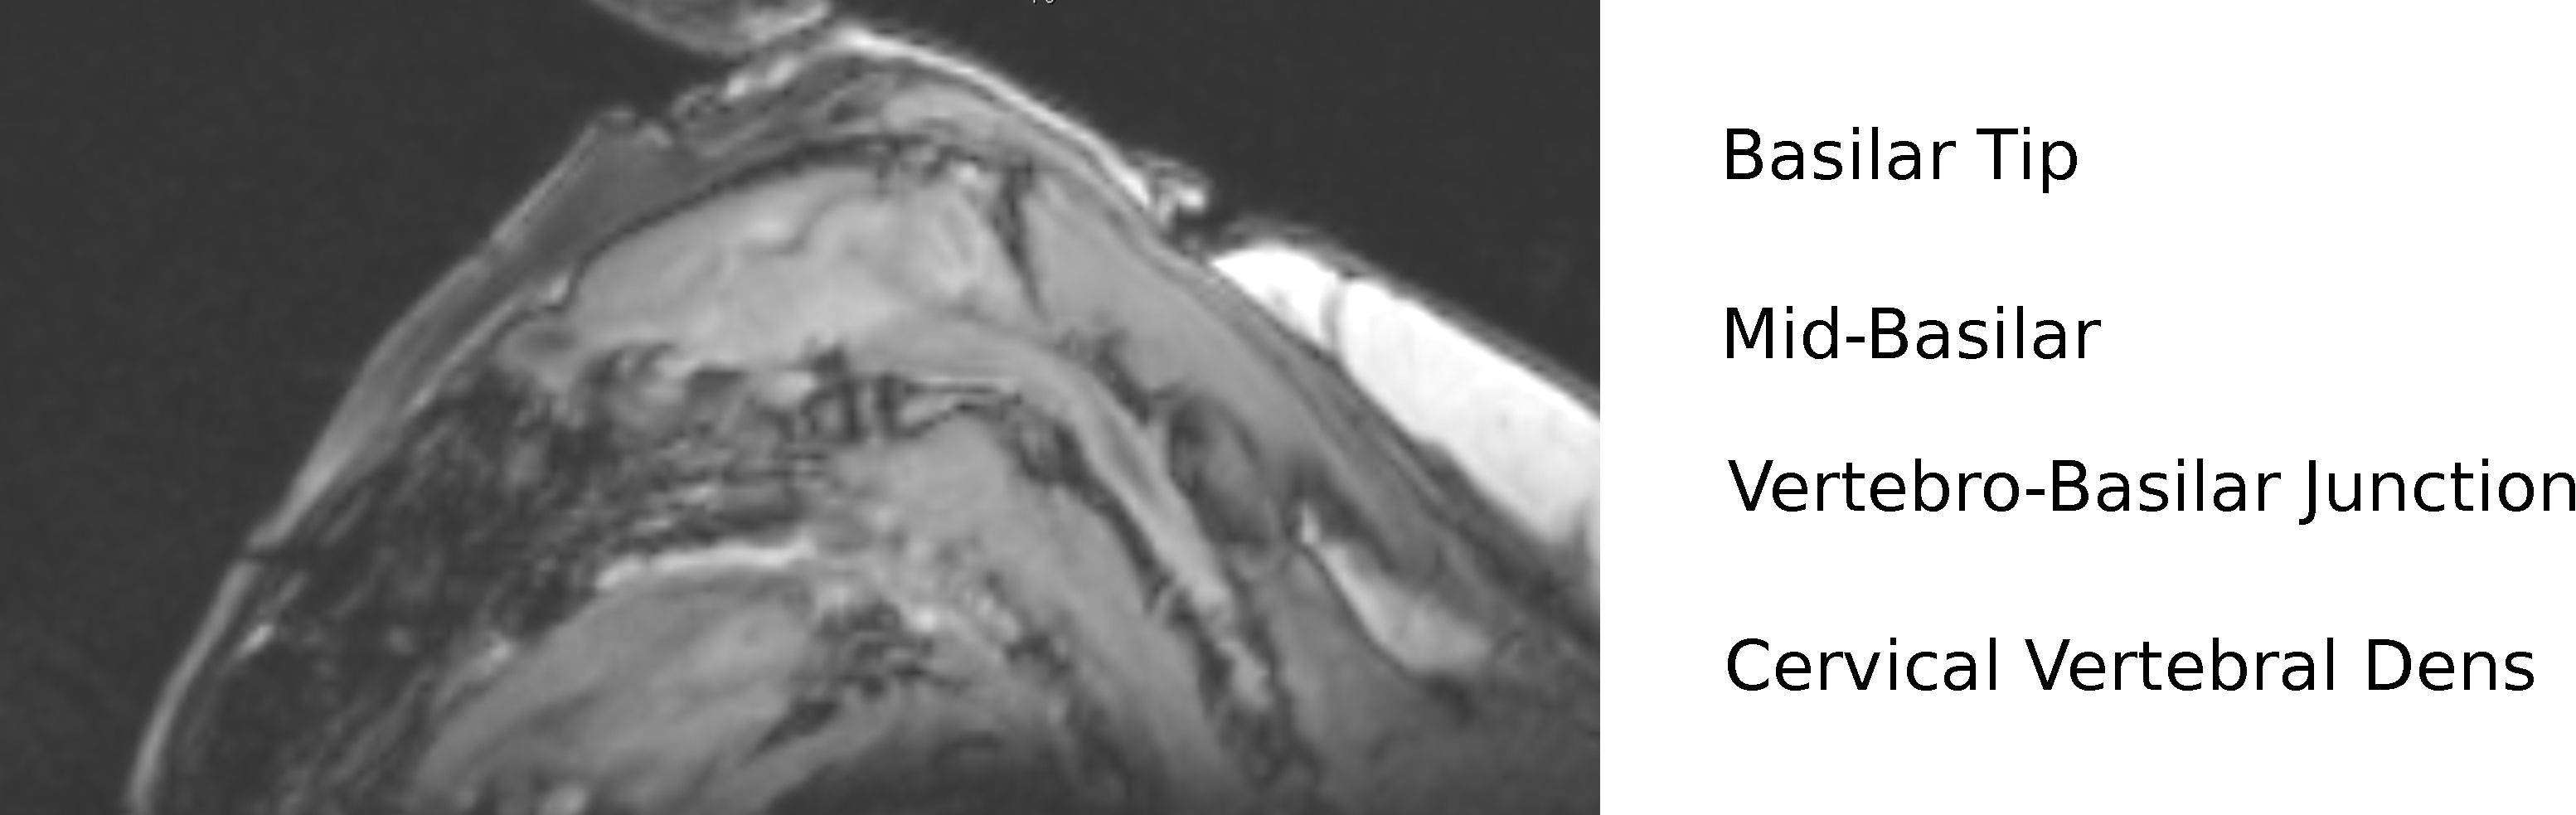
\includegraphics[height=0.75in]{brain.pdf}}
%\hspace*{.2in}
%\raisebox{-0.5\height}{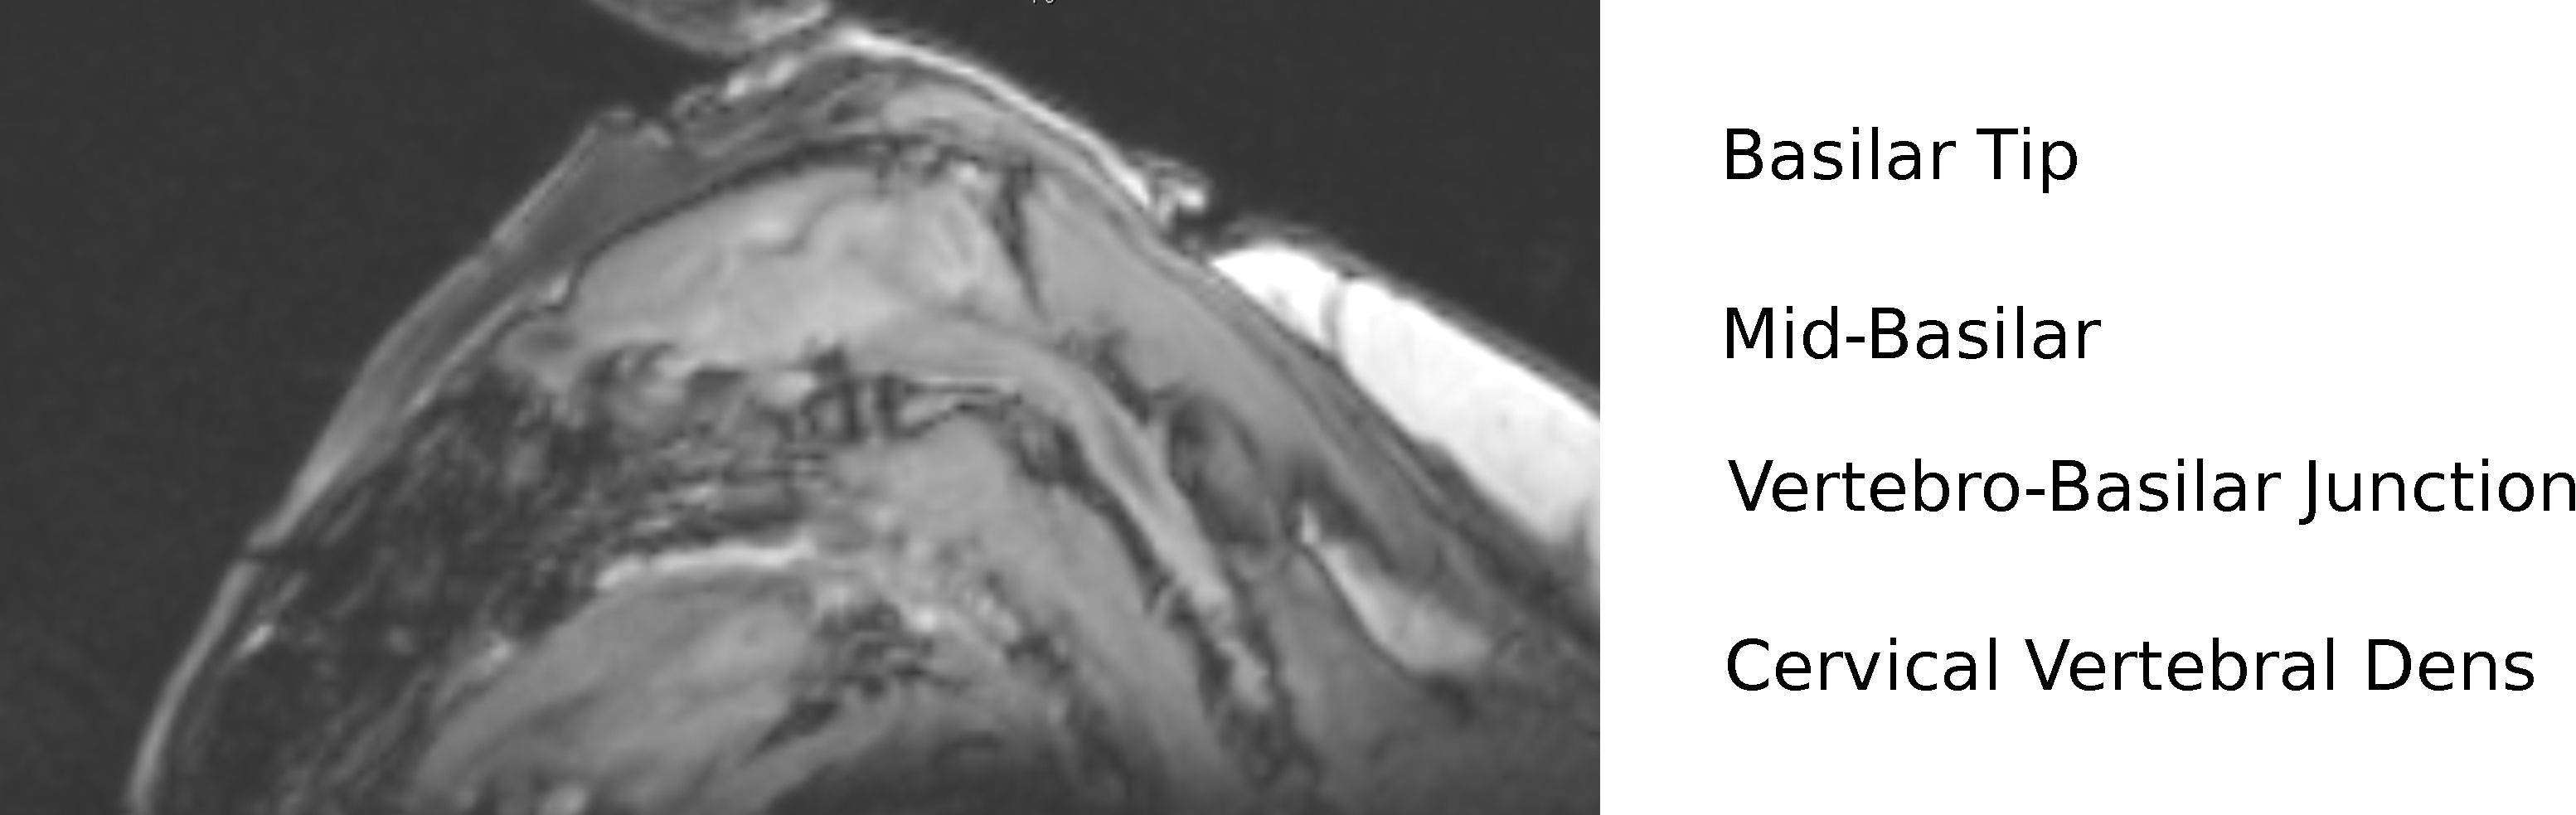
\includegraphics[height=0.3in]{brain.pdf}}
%\end{minipage}

\begin{figure}[H]
\begin{center}
\raisebox{-0.5\height}{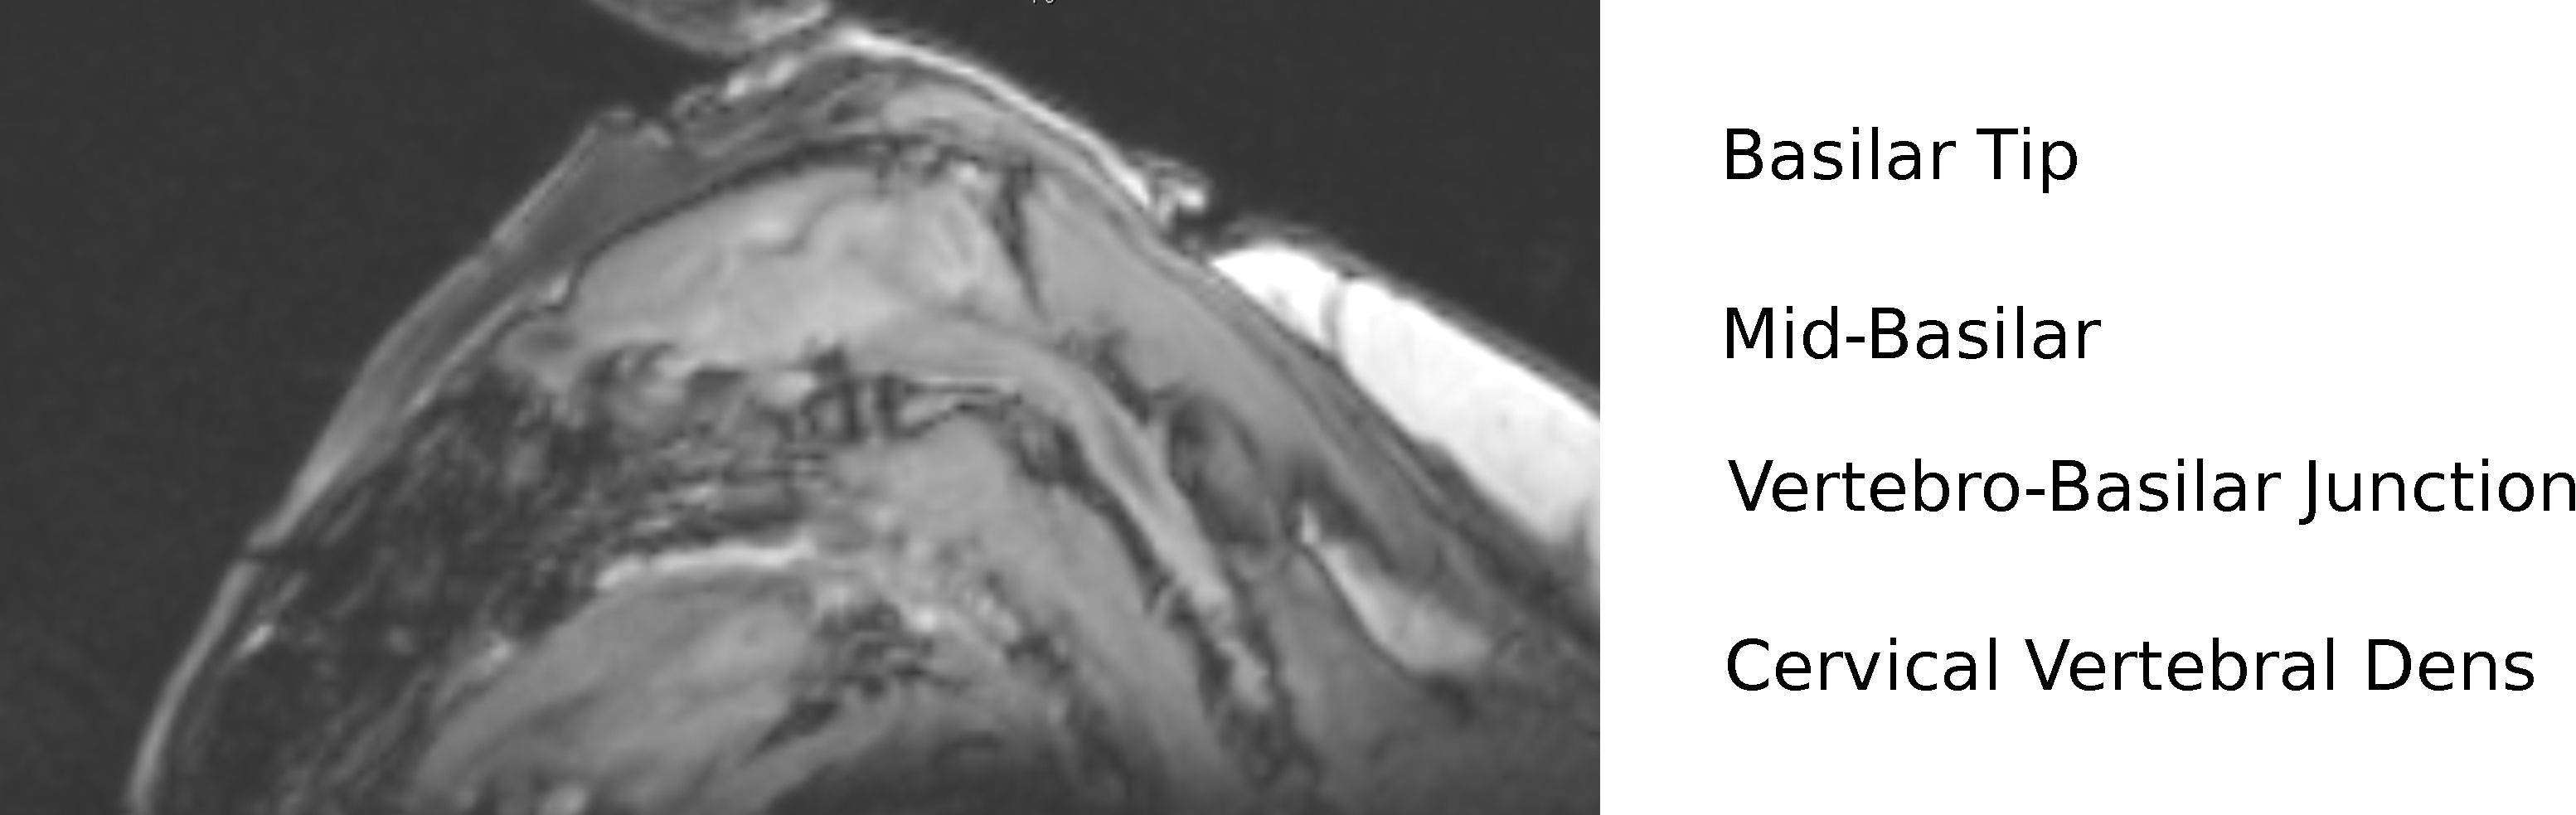
\includegraphics[scale=0.2]{brain.pdf}}
\hspace{0.2cm}
\raisebox{-0.5\height}{\includegraphics[scale=1.0]{../config/legend.pdf}} \\
\vspace{0.5cm}
\begin{tabular}{ccc}
& VEP On Response & VEP Off Response \\
\rotatebox{90}{\hspace{0.5cm}Basilar Tip} &
\includegraphics[scale=0.161]{../vep/matlab_data/_Thu_15_05_2014_11_57_42_vep_.pdf} &
\includegraphics[scale=0.161]{../vep/matlab_data/_Thu_15_05_2014_11_57_42_vep__off.pdf} \\
\rotatebox{90}{\hspace{0.5cm}Mid-Basilar} &
\includegraphics[scale=0.161]{../vep/matlab_data/_Thu_15_05_2014_14_13_26_vep_.pdf} &
\includegraphics[scale=0.161]{../vep/matlab_data/_Thu_15_05_2014_14_13_26_vep__off.pdf} \\
\rotatebox{90}{\hspace{0.5cm}Vertebro-basilar} &
\includegraphics[scale=0.161]{../vep/matlab_data/_Thu_15_05_2014_15_54_54_vep_.pdf} &
\includegraphics[scale=0.161]{../vep/matlab_data/_Thu_15_05_2014_15_54_54_vep__off.pdf} \\
\rotatebox{90}{\hspace{0.5cm}Basilar Tip} &
\includegraphics[scale=0.161]{../vep/matlab_data/_Thu_15_05_2014_16_47_47_vep_.pdf} &
\includegraphics[scale=0.161]{../vep/matlab_data/_Thu_15_05_2014_16_47_47_vep__off.pdf}
\end{tabular}
\caption{Rabbit 10 experimental VEP.}
\end{center}
\end{figure}

\begin{figure}[H]
\begin{center}
\begin{tabular}{cc}
VEP On Response & VEP Off Response \\
\includegraphics[scale=0.161]{../vep/matlab_data/_Thu_15_05_2014_12_15_47_vep_ctr.pdf} &
\includegraphics[scale=0.161]{../vep/matlab_data/_Thu_15_05_2014_12_15_47_vep_ctr_off.pdf}
\end{tabular}
\caption{Rabbit 10 live control VEP.}
\end{center}
\end{figure}

\begin{figure}[H]
\begin{center}
\begin{tabular}{cc}
VEP On Response & VEP Off Response \\
\includegraphics[scale=0.161]{../vep/matlab_data/_Thu_15_05_2014_17_22_22_vep_.pdf} &
\includegraphics[scale=0.161]{../vep/matlab_data/_Thu_15_05_2014_17_22_22_vep__off.pdf}
\end{tabular}
\caption{Rabbit 10 dead control VEP.}
\end{center}
\end{figure}

\begin{figure}[H]
\begin{center}
\begin{tabular}{cc}
VEP On Response & VEP Off Response \\
\includegraphics[scale=0.161]{../vep/matlab_data/_Thu_15_05_2014_09_55_41_vep_.pdf}
\includegraphics[scale=0.161]{../vep/matlab_data/_Thu_15_05_2014_09_55_41_vep__off.pdf} &
\end{tabular}
\caption{Rabbit 10 baseline VEP.}
\end{center}
\end{figure}

\begin{figure}[H]
\begin{center}
\raisebox{-0.5\height}{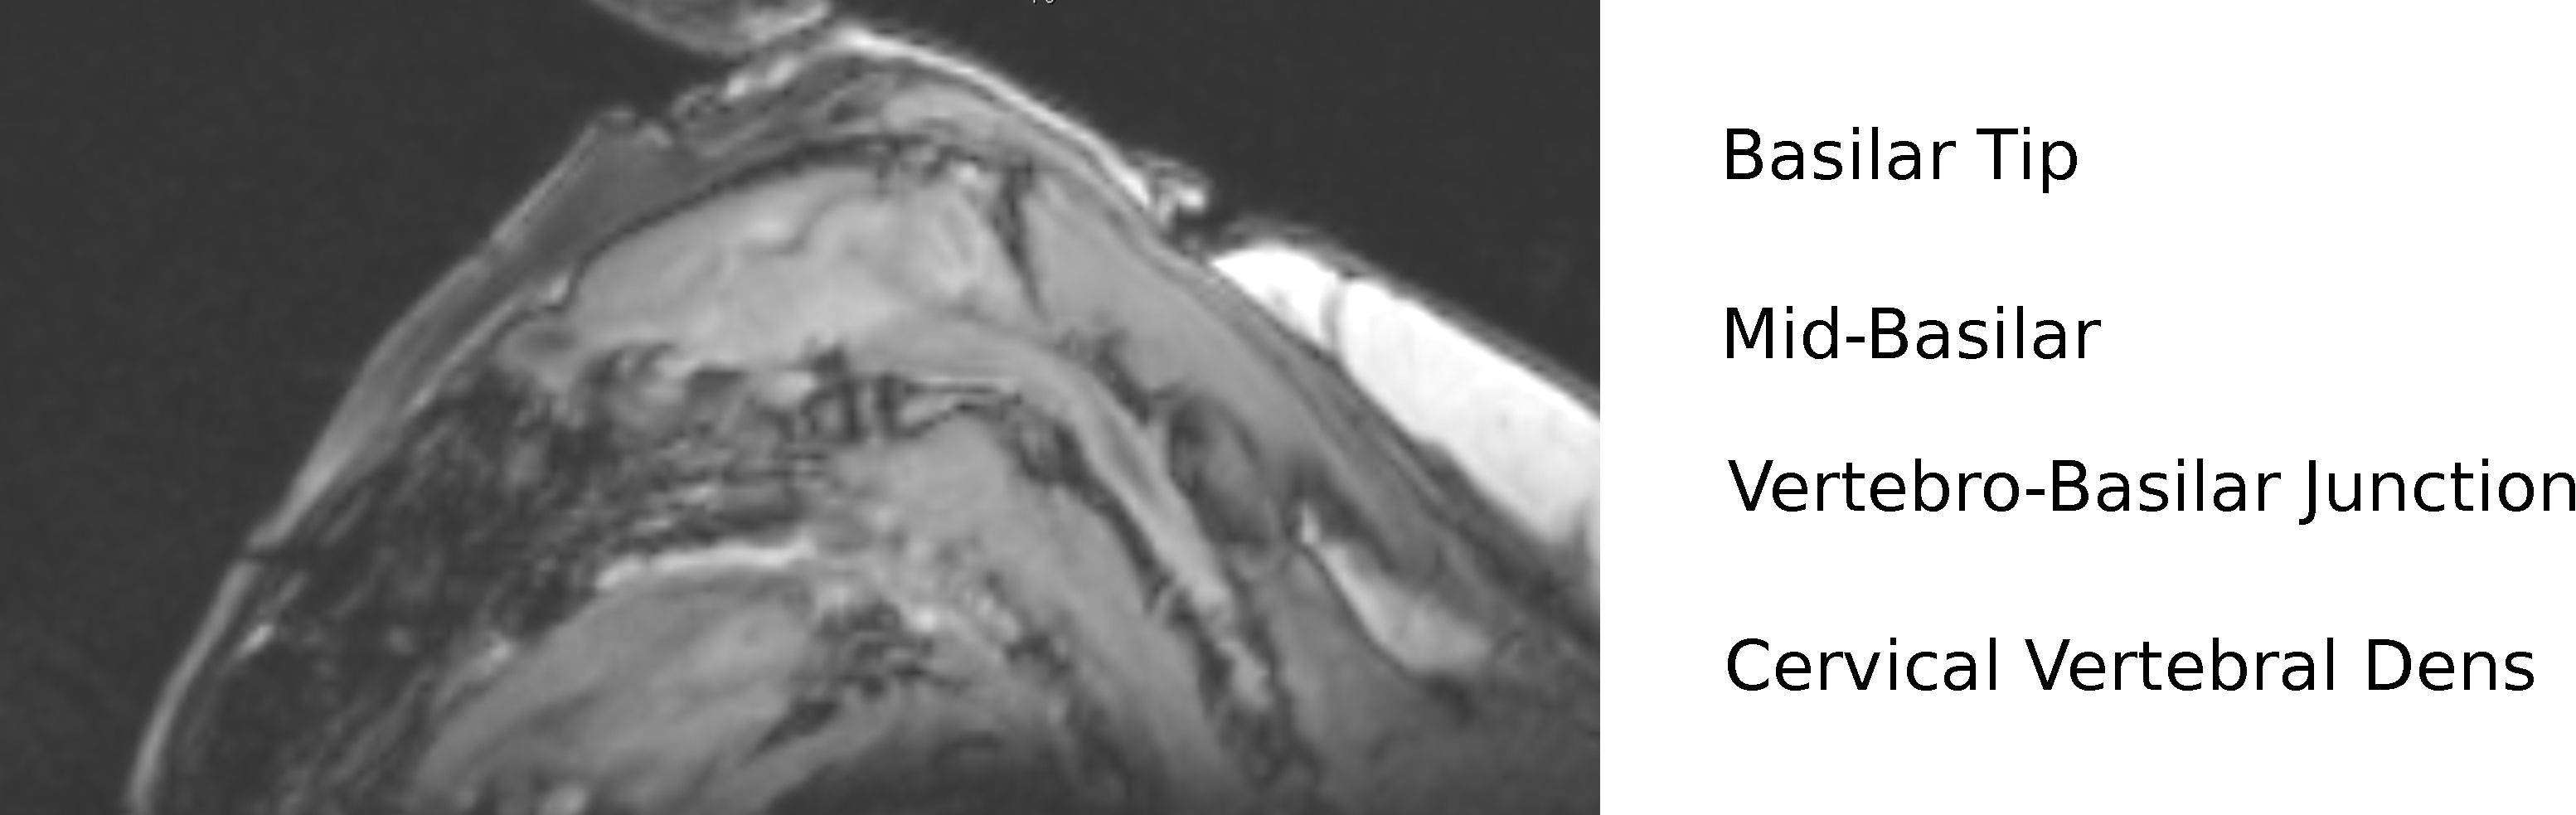
\includegraphics[scale=0.2]{brain.pdf}}
\hspace{0.2cm}
\raisebox{-0.5\height}{\includegraphics[scale=1.0]{../config/legend.pdf}} \\
\vspace{0.5cm}
\begin{tabular}{ccc}
& SSVEP 40 Hz & SSAEP 86 Hz \\
\rotatebox{90}{\hspace{0.5cm}Basilar Tip} &
\includegraphics[scale=0.161]{../ssavep/matlab_data/_Thu_15_05_2014_12_08_22_ssvep_40.pdf} &
\includegraphics[scale=0.161]{../ssavep/matlab_data/_Thu_15_05_2014_12_31_02_ssaep_86.pdf} \\
\rotatebox{90}{\hspace{0.5cm}Mid-Basilar} &
\includegraphics[scale=0.161]{../ssavep/matlab_data/_Thu_15_05_2014_14_20_24_ssvep_40.pdf} &
\includegraphics[scale=0.161]{../ssavep/matlab_data/_Thu_15_05_2014_14_26_54_ssaep_86.pdf} \\
\rotatebox{90}{\hspace{0.5cm}Vertebro-basilar} &
\includegraphics[scale=0.161]{../ssavep/matlab_data/_Thu_15_05_2014_16_02_44_ssvep_40.pdf} &
\includegraphics[scale=0.161]{../ssavep/matlab_data/_Thu_15_05_2014_16_12_19_ssaep_86.pdf} \\
\rotatebox{90}{\hspace{0.5cm}Basilar Tip} &
\includegraphics[scale=0.161]{../ssavep/matlab_data/_Thu_15_05_2014_16_38_47_ssvep_40.pdf} &
\includegraphics[scale=0.161]{../ssavep/matlab_data/_Thu_15_05_2014_16_58_34_ssaep_86.pdf}
\end{tabular}
\caption{Rabbit 10 experimental responses.}
\end{center}
\end{figure}

\begin{figure}[H]
\begin{center}
\begin{tabular}{cccc}
SSVEP 40 Hz & SSAEP 86 Hz \\
\includegraphics[scale=0.161]{../ssavep/matlab_data/_Thu_15_05_2014_12_13_26_ssvep_ctr_40.pdf} &
\includegraphics[scale=0.161]{../ssavep/matlab_data/_Thu_15_05_2014_12_26_26_ssaep_ctr_86.pdf}
\end{tabular}
\caption{Rabbit 10 live control.}
\end{center}
\end{figure}

\begin{figure}[H]
\begin{center}
\begin{tabular}{cccc}
SSVEP 40 Hz & SSAEP 86 Hz \\
\includegraphics[scale=0.161]{../ssavep/matlab_data/_Thu_15_05_2014_17_18_01_ssvep_40.pdf} &
\includegraphics[scale=0.161]{../ssavep/matlab_data/_Thu_15_05_2014_17_12_38_ssaep_86.pdf}
\end{tabular}
\caption{Rabbit 10 dead control.}
\end{center}
\end{figure}


\begin{figure}[H]
\begin{center}
\begin{tabular}{cccc}
SSVEP 40 Hz & SSAEP 86 Hz \\
\includegraphics[scale=0.161]{../ssavep/matlab_data/_Thu_15_05_2014_09_52_53_ssvep_40.pdf} &
\includegraphics[scale=0.161]{../ssavep/matlab_data/_Thu_15_05_2014_10_04_16_ssaep_86.pdf}
\end{tabular}
\caption{Rabbit 10 baseline.}
\end{center}
\end{figure}

\begin{figure}[H]
\begin{center}
\raisebox{-0.5\height}{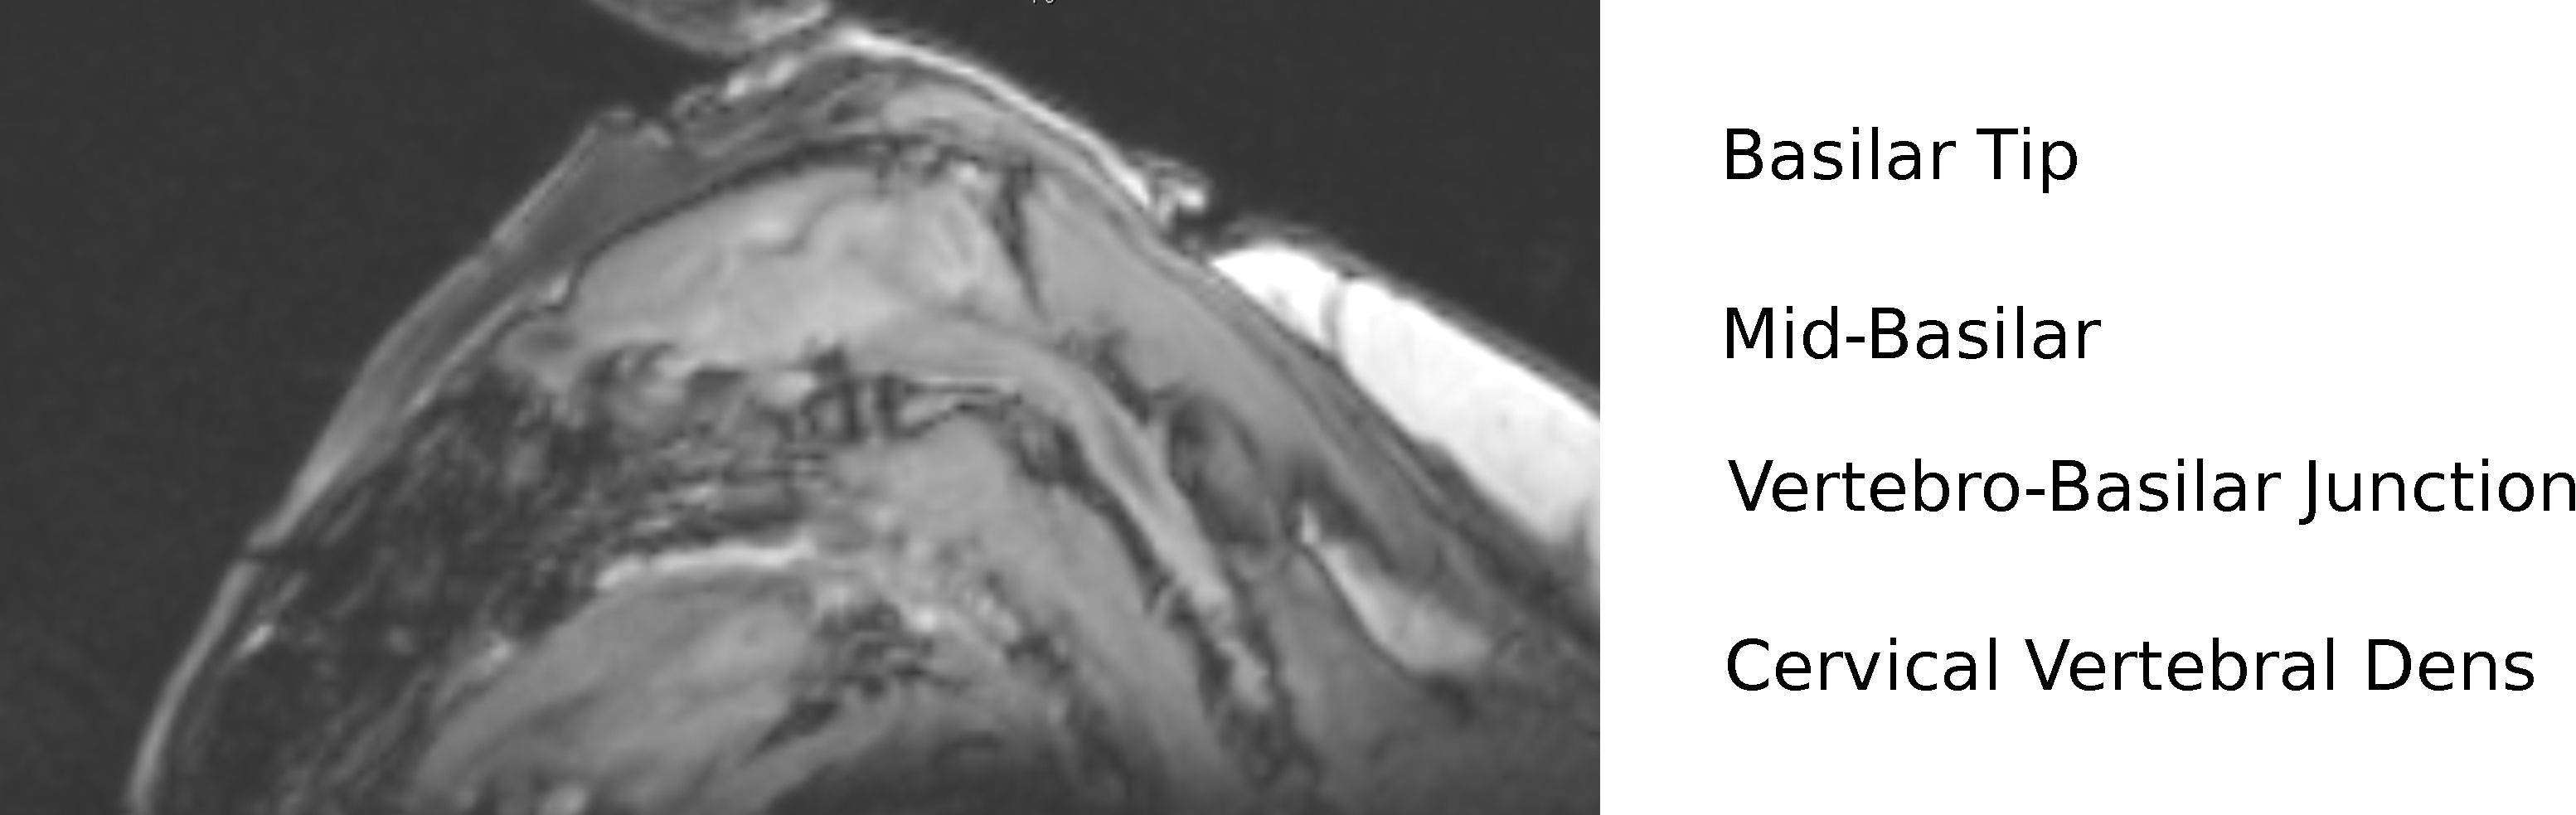
\includegraphics[scale=0.2]{brain.pdf}}
\hspace{0.2cm}
\raisebox{-0.5\height}{\includegraphics[scale=1.0]{../config/legend.pdf}} \\
\vspace{0.5cm}
\begin{tabular}{ccc}
& VEP On Response & VEP Off Response \\
\rotatebox{90}{\hspace{0.5cm}Basilar Tip} &
\includegraphics[scale=0.161]{../vep/matlab_data/_Tue_06_05_2014_11_17_10_vep_.pdf} &
\includegraphics[scale=0.161]{../vep/matlab_data/_Tue_06_05_2014_11_17_10_vep__off.pdf} \\
\rotatebox{90}{\hspace{0.5cm}Mid-Basilar} &
\includegraphics[scale=0.161]{../vep/matlab_data/_Tue_06_05_2014_14_04_18_vep_.pdf} &
\includegraphics[scale=0.161]{../vep/matlab_data/_Tue_06_05_2014_14_04_18_vep__off.pdf} \\
\rotatebox{90}{\hspace{0.5cm}Vertebro-basilar} &
\includegraphics[scale=0.161]{../vep/matlab_data/_Tue_06_05_2014_14_44_57_vep_.pdf} &
\includegraphics[scale=0.161]{../vep/matlab_data/_Tue_06_05_2014_14_44_57_vep__off.pdf} \\
%\rotatebox{90}{\hspace{0cm}Cervical Vertebral Dens} &
%\includegraphics[scale=0.161]{../vep/matlab_data/_Tue_06_05_2014_15_13_50_vep_.pdf} &
%\includegraphics[scale=0.161]{../vep/matlab_data/_Tue_06_05_2014_15_13_50_vep__off.pdf} \\
\rotatebox{90}{\hspace{0.5cm}Basilar Tip} &
\includegraphics[scale=0.161]{../vep/matlab_data/_Tue_06_05_2014_15_50_43_vep_.pdf} &
\includegraphics[scale=0.161]{../vep/matlab_data/_Tue_06_05_2014_15_50_43_vep__off.pdf}
\end{tabular}
\caption{Rabbit 9 experimental responses.}
\end{center}
\end{figure}

\begin{figure}[H]
\begin{center}
\begin{tabular}{cc}
VEP On Response & VEP Off Response \\
\includegraphics[scale=0.161]{../vep/matlab_data/_Tue_06_05_2014_11_25_22_vep_.pdf} &
\includegraphics[scale=0.161]{../vep/matlab_data/_Tue_06_05_2014_11_25_22_vep__off.pdf}
\end{tabular}
\caption{Rabbit 9 live control VEP.}
\end{center}
\end{figure}

\begin{figure}[H]
\begin{center}
\begin{tabular}{cc}
VEP On Response & VEP Off Response \\
\includegraphics[scale=0.161]{../vep/matlab_data/_Tue_06_05_2014_09_55_56_vep_3m.pdf}
\includegraphics[scale=0.161]{../vep/matlab_data/_Tue_06_05_2014_09_55_56_vep_3m_off.pdf} &
\end{tabular}
\caption{Rabbit 9 baseline VEP.}
\end{center}
\end{figure}

\begin{figure}[H]
\begin{center}
\raisebox{-0.5\height}{\includegraphics[scale=0.2]{brain.pdf}}
\hspace{0.2cm}
\raisebox{-0.5\height}{\includegraphics[scale=1.0]{../config/legend.pdf}} \\
\vspace{0.5cm}
\begin{tabular}{ccc}
& SSVEP 40 Hz & SSAEP 86 Hz \\
\rotatebox{90}{\hspace{0.5cm}Basilar Tip} &
\includegraphics[scale=0.161]{../ssavep/matlab_data/_Tue_06_05_2014_11_14_51_ssvep_40.pdf} &
\includegraphics[scale=0.161]{../ssavep/matlab_data/_Tue_06_05_2014_11_37_22_ssaep_86.pdf} \\
\rotatebox{90}{\hspace{0.5cm}Mid-Basilar} &
\includegraphics[scale=0.161]{../ssavep/matlab_data/_Tue_06_05_2014_14_02_01_ssvep_40.pdf} &
\includegraphics[scale=0.161]{../ssavep/matlab_data/_Tue_06_05_2014_14_11_09_ssaep_86.pdf} \\
\rotatebox{90}{\hspace{0.5cm}Vertebro-basilar} &
\includegraphics[scale=0.161]{../ssavep/matlab_data/_Tue_06_05_2014_14_41_46_ssvep_40.pdf} &
\includegraphics[scale=0.161]{../ssavep/matlab_data/_Tue_06_05_2014_14_53_21_ssaep_86.pdf} \\
%\rotatebox{90}{\hspace{0cm}Cervical Vertebral Dens} &
%\includegraphics[scale=0.161]{../ssavep/matlab_data/_Tue_06_05_2014_15_11_25_ssvep_40.pdf} &
%\includegraphics[scale=0.161]{../ssavep/matlab_data/_Tue_06_05_2014_15_20_29_ssaep_86.pdf} \\
\rotatebox{90}{\hspace{0.5cm}Basilar Tip} &
\includegraphics[scale=0.161]{../ssavep/matlab_data/_Tue_06_05_2014_15_48_24_ssvep_50.pdf} &
\includegraphics[scale=0.161]{../ssavep/matlab_data/_Tue_06_05_2014_15_57_52_ssaep_86.pdf}
\end{tabular}
\caption{Rabbit 9 experimental responses.}
\end{center}
\end{figure}

\begin{figure}[H]
\begin{center}
\begin{tabular}{cc}
SSVEP 40 Hz & SSAEP 86 Hz \\
\includegraphics[scale=0.161]{../ssavep/matlab_data/_Tue_06_05_2014_11_23_01_ssvep_40.pdf} &
\includegraphics[scale=0.161]{../ssavep/matlab_data/_Tue_06_05_2014_11_42_15_ssaep_86.pdf}
\end{tabular}
\caption{Rabbit 9 live control.}
\end{center}
\end{figure}

\begin{figure}[H]
\begin{center}
\begin{tabular}{cc}
SSVEP 40 Hz & SSAEP 86 Hz \\
\includegraphics[scale=0.161]{../ssavep/matlab_data/_Tue_06_05_2014_09_52_56_ssvep_40.pdf} &
\includegraphics[scale=0.161]{../ssavep/matlab_data/_Tue_06_05_2014_10_08_48_ssaep_86.pdf}
\end{tabular}
\caption{Rabbit 9 baseline.}
\end{center}
\end{figure}



\end{document}

